% !TeX spellcheck = ru_RU
% !TEX root = vkr.tex

\section{Результаты экспериментов и их анализ} \label{sec:experiment}

В данном разделе приводятся результаты экспериментальной оценки 12~моделей на двух независимых бенчмарках: \texttt{benchmark-combined} (500~примеров: 326~GEO / 174~TAG) и \texttt{benchmark-real} (250~примеров: 203~GEO / 47~TAG). Методология подготовки данных и проведения экспериментов описана в разделе~\ref{sec:method}; определения метрик~--- в разделе~\ref{sec:background}.

%%% ============================================================
\subsection{Оценка базовой модели} \label{subsec:baseline}
%%% ============================================================

Базовой линией (baseline) служит модель YandexGPT~5.1~Pro без дообучения (\texttt{pro\_baseline}). Результаты представлены в таблице~\ref{tab:baseline_results}.

\begin{table}[H]
\centering
\caption{Метрики базовой модели \texttt{pro\_baseline} на двух бенчмарках. 95\%~bootstrap-CI для error rate построен перцентильным методом ($B = 1000$, $\mathrm{seed} = 42$). $n_\mathrm{err}$~--- общее число неверных ответов (incorrect $+$ $\rho_\varnothing$).}
\label{tab:baseline_results}
\def\arraystretch{1.15}
\setlength\tabcolsep{0.4em}
\begin{tabular}{l r l r r r}
    \toprule
    \textbf{Бенчмарк} & \textbf{ER} & \textbf{95\%~CI} & \textbf{Macro~F1} & $\boldsymbol{n_\mathrm{err}}$ & $\boldsymbol{\rho_\varnothing}$ \\
    \midrule
    combined (500) & $0{,}182$ & $[0{,}148;\,0{,}216]$ & $0{,}526$ & 91 & $6{,}8\%$ \\
    real (250)     & $0{,}172$ & $[0{,}128;\,0{,}216]$ & $0{,}617$ & 43 & $6{,}0\%$ \\
    \bottomrule
\end{tabular}
\end{table}

Низкое значение Macro~$F_1 = 0{,}526$ при error rate $18{,}2\%$ указывает на выраженный дисбаланс качества между классами. Анализ матрицы ошибок выявляет систематический паттерн: все 57~ошибок типа TAG$\to$GEO, ни одного обратного случая (GEO$\to$TAG); ещё 34~запроса не получают \texttt{tool\_call} вовсе ($\rho_\varnothing = 6{,}8\%$). Дополнительно: из 174~запросов класса TAG корректно классифицированы лишь 86~($49{,}4\%$~recall). Базовая модель по умолчанию предпочитает вызов \texttt{ResolveEntities} (GEO) как более общий, что и порождает наблюдаемый bias и непригодность для промышленного применения без адаптации.

%%% ============================================================
\subsection{Основные результаты дообучения} \label{subsec:main_results}
%%% ============================================================

Результаты всех 12~моделей на \texttt{benchmark-combined} приведены в таблице~\ref{tab:combined_results}. Модели различаются по типу и объёму обучающих данных.

\begin{table}[H]
\centering
\caption{Результаты на \texttt{benchmark-combined} (500 примеров: 326~GEO / 174~TAG). 95\%~bootstrap-CI для error rate~--- перцентильный метод, $B = 1000$, $\mathrm{seed} = 42$; $n_\mathrm{err}$~--- общее число неверных ответов (incorrect $+$ $\rho_\varnothing$); $\rho_\varnothing$~--- доля ответов без \texttt{tool\_call}.}
\label{tab:combined_results}
\def\arraystretch{1.15}
\setlength\tabcolsep{0.25em}
{\small
\begin{tabular}{l l r l r r r}
    \toprule
    \textbf{Модель} & \textbf{Обуч. данные} & \textbf{ER} & \textbf{95\%~CI} & \textbf{M-F1} & $\boldsymbol{n_\mathrm{err}}$ & $\boldsymbol{\rho_\varnothing}$ \\
    \midrule
    pro\_baseline       & --- (без тюна)    & $0{,}182$ & $[0{,}148;\,0{,}216]$ & .526 & 91 & $6{,}8\%$ \\
    \midrule
    lite\_latest\_v1    & Синт.\,${\sim}$1500 & $0{,}072$ & $[0{,}052;\,0{,}096]$ & .925 & 36 & $0{,}4\%$ \\
    lite\_latest\_v2    & Синт.\,${\sim}$1500 & $0{,}016$ & $[0{,}006;\,0{,}028]$ & .985 &  8 & $0{,}4\%$ \\
    lite\_latest\_v3    & Синт.\,${\sim}$1500 & $0{,}034$ & $[0{,}018;\,0{,}050]$ & .966 & 17 & $0{,}4\%$ \\
    \midrule
    lite\_rc\_v1        & Синт.\,${\sim}$1500 & $0{,}020$ & $[0{,}008;\,0{,}034]$ & .981 & 10 & $0{,}4\%$ \\
    lite\_rc\_v2        & Синт.\,${\sim}$1500 & $0{,}026$ & $[0{,}012;\,0{,}042]$ & .974 & 13 & $0{,}4\%$ \\
    \midrule
    train\_synth\_50    & Синт.\,50        & $0{,}054$ & $[0{,}036;\,0{,}074]$ & .631 & 27 & $0{,}4\%$ \\
    train\_synth\_250   & Синт.\,250       & $0{,}054$ & $[0{,}036;\,0{,}074]$ & .945 & 27 & $0{,}4\%$ \\
    train\_synth\_500   & Синт.\,500       & $0{,}022$ & $[0{,}010;\,0{,}036]$ & .979 & 11 & $0{,}4\%$ \\
    train\_synth\_1000  & Синт.\,908       & $0{,}044$ & $[0{,}026;\,0{,}062]$ & .955 & 22 & $0{,}4\%$ \\
    \midrule
    train\_real\_250    & Реал.\,250         & $0{,}048$ & $[0{,}030;\,0{,}068]$ & .949 & 24 & $0{,}4\%$ \\
    train\_mixed\_500   & Микс\,500          & $0{,}006$ & $[0{,}000;\,0{,}014]$ & .996 &  3 & $0{,}4\%$ \\
    \bottomrule
\end{tabular}
}
\end{table}

\begin{figure}[H]
\centering

\includegraphics[width=0.95\textwidth]{figures/accuracy_ci.png}
\caption{Error rate всех 12~моделей на \texttt{benchmark-combined} с 95\%~bootstrap-доверительными интервалами. Горизонтальная линия~--- целевое значение~$0{,}10$.}
\label{fig:accuracy_ci}
\end{figure}

Ключевые наблюдения:
\begin{enumerate}
    \item \textbf{Снижение error rate на два порядка.} У лучшей дообученной модели \texttt{train\_mixed\_500} error rate снижается с $0{,}182$ (baseline) до $0{,}006$~--- более чем в~$30$~раз, или относительно на $96{,}7\%$ ($91 \to 3$ ошибочных ответов из~500). Даже наименее успешная дообученная модель (\texttt{lite\_latest\_v1}, $\mathrm{ER} = 0{,}072$) снижает error rate более чем в~$2{,}5$~раза.

    \item \textbf{Эффект минимального объёма.} Уже 50~синтетических примеров снижают error rate с $0{,}182$ до $0{,}054$ ($\times 3{,}4$), что согласуется с~гипотезой~\ref{hyp:lora_significance} и аналогией поверхностного выравнивания~\cite{zhou2023lima}.

    \item \textbf{Устранение отказов.} Все дообученные модели снижают $\rho_\varnothing$ с $6{,}8\%$ (34~из~500) до $0{,}4\%$ (2~из~500).

    \item \textbf{Абсолютный лидер.} Модель \texttt{train\_mixed\_500}, обученная на сбалансированной комбинации реальных и синтетических данных (500~примеров), достигает $\mathrm{ER} = 0{,}006$ и Macro~$F_1 = 0{,}996$ с единственной ошибочной классификацией и двумя отказами.
\end{enumerate}

%%% ============================================================
\subsection{Валидация на реальных данных} \label{subsec:real_validation}
%%% ============================================================

Для оценки обобщающей способности моделей используется независимый бенчмарк \texttt{benchmark-real}, составленный из реальных пользовательских запросов. Результаты и разность с \texttt{benchmark-combined} приведены в таблице~\ref{tab:real_results}.

\begin{table}[H]
\centering
\caption{Результаты на \texttt{benchmark-real} (250 примеров: 203~GEO / 47~TAG). 95\%~bootstrap-CI~--- перцентильный метод, $B = 1000$, $\mathrm{seed} = 42$; $\rho_\varnothing$~--- доля ответов без \texttt{tool\_call}; $\Delta\mathrm{ER}$~--- разность с \texttt{benchmark-combined} (положительные значения~--- деградация).}
\label{tab:real_results}
\def\arraystretch{1.15}
\setlength\tabcolsep{0.25em}
{\small
\begin{tabular}{l r l r r r r}
    \toprule
    \textbf{Модель} & \textbf{ER} & \textbf{95\%~CI} & \textbf{M-F1} & $\boldsymbol{n_\mathrm{err}}$ & $\boldsymbol{\rho_\varnothing}$ & $\boldsymbol{\Delta}$\textbf{ER} \\
    \midrule
    pro\_baseline       & $0{,}172$ & $[0{,}128;\,0{,}216]$ & $0{,}617$ & 43 & $6{,}0\%$ & $-0{,}010$ \\
    \midrule
    lite\_latest\_v1    & $0{,}096$ & $[0{,}064;\,0{,}132]$ & $0{,}872$ & 24 & $0{,}8\%$ & $+0{,}024$ \\
    lite\_latest\_v2    & $0{,}032$ & $[0{,}012;\,0{,}056]$ & $0{,}959$ &  8 & $0{,}8\%$ & $+0{,}016$ \\
    lite\_latest\_v3    & $0{,}068$ & $[0{,}040;\,0{,}100]$ & $0{,}906$ & 17 & $0{,}8\%$ & $+0{,}034$ \\
    \midrule
    lite\_rc\_v1        & $0{,}052$ & $[0{,}028;\,0{,}084]$ & $0{,}921$ & 13 & $0{,}8\%$ & $+0{,}032$ \\
    lite\_rc\_v2        & $0{,}056$ & $[0{,}032;\,0{,}088]$ & $0{,}916$ & 14 & $0{,}8\%$ & $+0{,}030$ \\
    \midrule
    train\_synth\_50    & $0{,}096$ & $[0{,}064;\,0{,}132]$ & $0{,}584$ & 24 & $0{,}8\%$ & $+0{,}042$ \\
    train\_synth\_250   & $0{,}108$ & $[0{,}072;\,0{,}148]$ & $0{,}856$ & 27 & $0{,}8\%$ & $+0{,}054$ \\
    train\_synth\_500   & $0{,}044$ & $[0{,}020;\,0{,}072]$ & $0{,}942$ & 11 & $0{,}8\%$ & $+0{,}022$ \\
    train\_synth\_1000  & $0{,}088$ & $[0{,}056;\,0{,}124]$ & $0{,}882$ & 22 & $0{,}8\%$ & $+0{,}044$ \\
    \midrule
    train\_real\_250    & $0{,}020$ & $[0{,}004;\,0{,}040]$ & $0{,}978$ &  5 & $0{,}8\%$ & $-0{,}028$ \\
    train\_mixed\_500   & $0{,}012$ & $[0{,}000;\,0{,}028]$ & $0{,}991$ &  3 & $0{,}8\%$ & $+0{,}006$ \\
    \bottomrule
\end{tabular}
}
\end{table}

Столбец $\Delta\mathrm{ER}$ показывает разность error rate на \texttt{benchmark-real} и \texttt{benchmark-combined}. Модели, обученные исключительно на синтетических данных, демонстрируют устойчивый рост error rate на реальных данных в диапазоне $+2{,}2\ldots +5{,}4$~п.п. Это свидетельствует об ограниченной обобщающей способности синтетических данных: модели частично переобучаются на характерные паттерны генерации, отсутствующие в реальных запросах.

Модель \texttt{train\_real\_250}, обученная на 250 реальных примерах, напротив, демонстрирует снижение error rate на $-2{,}8$~п.п.\ при переходе на реальный бенчмарк, что объяснимо совпадением распределений обучающей и тестовой выборок.

Модель \texttt{train\_mixed\_500} показывает минимальную деградацию: $\Delta\mathrm{ER} = +0{,}006$, что свидетельствует о высокой робастности, достигаемой за счёт сочетания разнородных обучающих данных. На самом~real\nobreakdash-бенчмарке её error rate составляет $0{,}012$~--- снижение в~$14$~раз относительно baseline ($0{,}172$).

\begin{figure}[H]
\centering
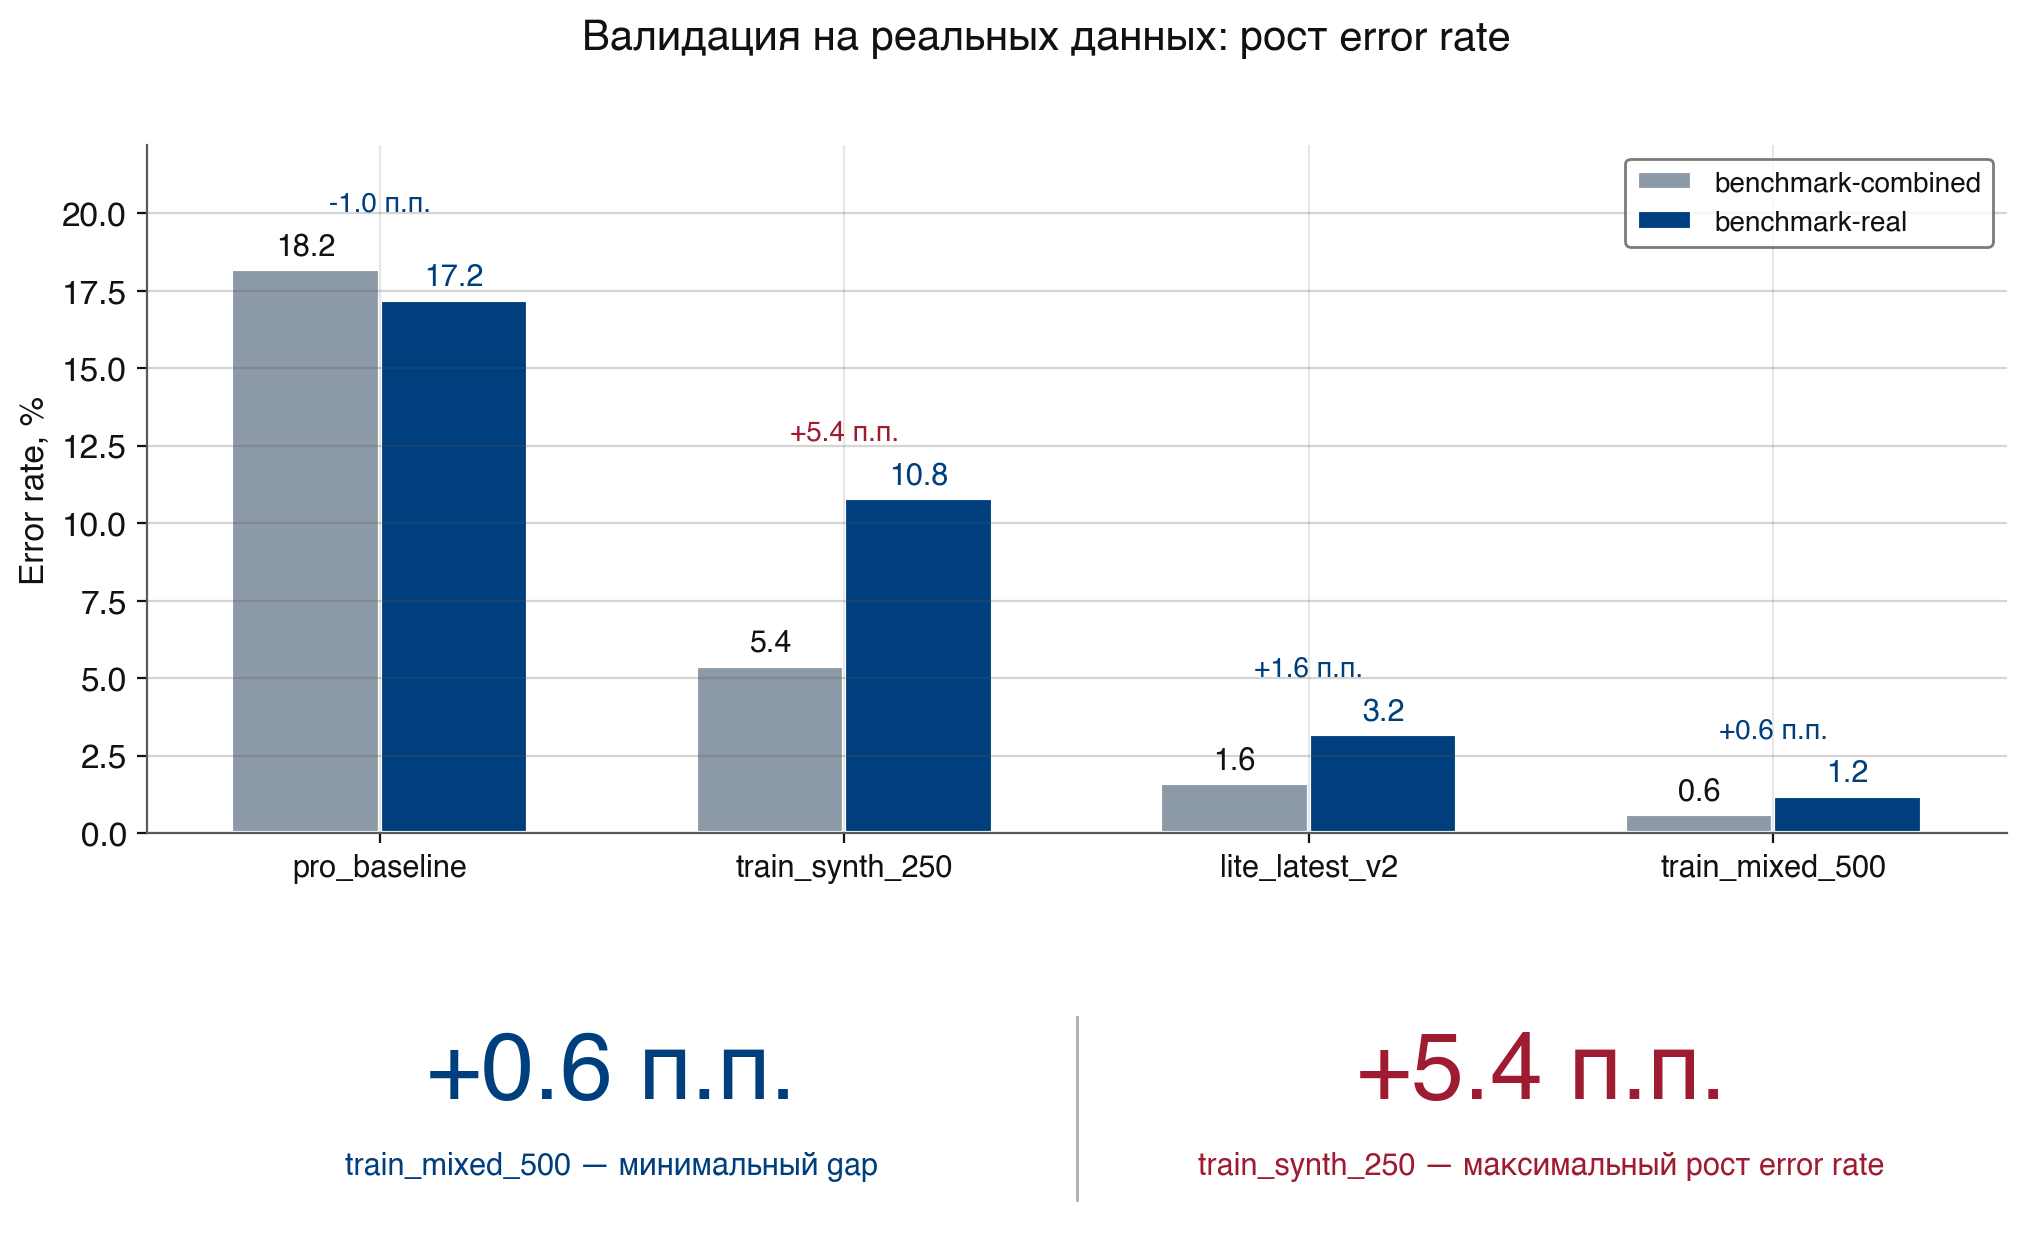
\includegraphics[width=0.9\textwidth]{figures/generalization_gap.png}
\caption{Обобщающий разрыв: $\Delta\mathrm{ER}$ при переходе с \texttt{benchmark-combined} на \texttt{benchmark-real}. Положительные значения~--- деградация (рост error rate) на реальных данных.}
\label{fig:generalization_gap}
\end{figure}

%%% ============================================================
\subsection{Анализ кривой обучения} \label{subsec:learning_curve}
%%% ============================================================

Для исследования зависимости качества от объёма обучающих данных (RQ2) обучена серия моделей на синтетических выборках объёмом 50, 250, 500 и 908~примеров. Результаты на \texttt{benchmark-combined} представлены в таблице~\ref{tab:learning_curve}.

\begin{table}[H]
\centering
\caption{Кривая обучения: зависимость метрик от объёма синтетических данных на \texttt{benchmark-combined}. 95\%~bootstrap-CI ($B = 1000$, $\mathrm{seed} = 42$, перцентильный метод).}
\label{tab:learning_curve}
\def\arraystretch{1.15}
\setlength\tabcolsep{0.5em}
\begin{tabular}{r r l r}
    \toprule
    \textbf{Объём} & \textbf{Error rate} & \textbf{95\%~CI} & \textbf{Macro~F1} \\
    \midrule
    50  & $0{,}054$ & $[0{,}036;\,0{,}074]$ & $0{,}631$ \\
    250 & $0{,}054$ & $[0{,}036;\,0{,}074]$ & $0{,}945$ \\
    500 & $0{,}022$ & $[0{,}010;\,0{,}036]$ & $0{,}979$ \\
    908 & $0{,}044$ & $[0{,}026;\,0{,}062]$ & $0{,}955$ \\
    \bottomrule
\end{tabular}
\end{table}

Кривая обучения обнаруживает нетривиальный немонотонный характер:
\begin{enumerate}
    \item \textbf{Разрыв error rate и Macro~$F_1$ при 50~примерах.} При одинаковом error rate ($0{,}054$) на 50 и 250~примерах Macro~$F_1$ возрастает с~$0{,}631$ до~$0{,}945$. Этот разрыв объясняется не деградацией распознавания, а артефактом macro-усреднения. Анализ confusion matrix модели \texttt{train\_synth\_50} (таблица~\ref{tab:confusion_synth50}) показывает, что в 2~случаях из 500 модель генерирует вызов \emph{несуществующего} инструмента \texttt{GetSearchQuerySummary}~--- побочный продукт недоученной модели, не покрывшей всё пространство допустимых токенов. В отчёте оценщика этот лейбл фиксируется как третий класс с $\mathrm{support} = 0$ и $F_1 = 0$, что тянет среднее вниз:
    \[
        \mathrm{Macro}\,F_1 = (0 + 0{,}959 + 0{,}934)/3 = 0{,}631.
    \]
    На 250~примерах паразитный класс исчезает, оценщик возвращается к двум лейблам, и Macro~$F_1$ нормализуется до~$0{,}945$. Таким образом, уже 50~примеров достаточно для устранения основного bias baseline, однако минимум ${\sim}\,250$~примеров необходимо для устойчивого подавления генерации несуществующих имён инструментов.

    \item \textbf{Минимум error rate на 500~примерах.} Лучший результат среди синтетических моделей: $\mathrm{ER} = 0{,}022$, Macro~$F_1 = 0{,}979$.

    \item \textbf{Деградация при увеличении до 908 примеров.} Дальнейшее наращивание объёма приводит к росту error rate до~$0{,}044$ ($+2{,}2$~п.п., рост ошибки в~$2$~раза). Эффект объясняется переобучением на артефакты синтетической генерации: с ростом объёма выборки доля повторяющихся шаблонов увеличивается, и модель начинает эксплуатировать статистические закономерности, специфичные для синтетического распределения.
\end{enumerate}

\begin{figure}[H]
\centering
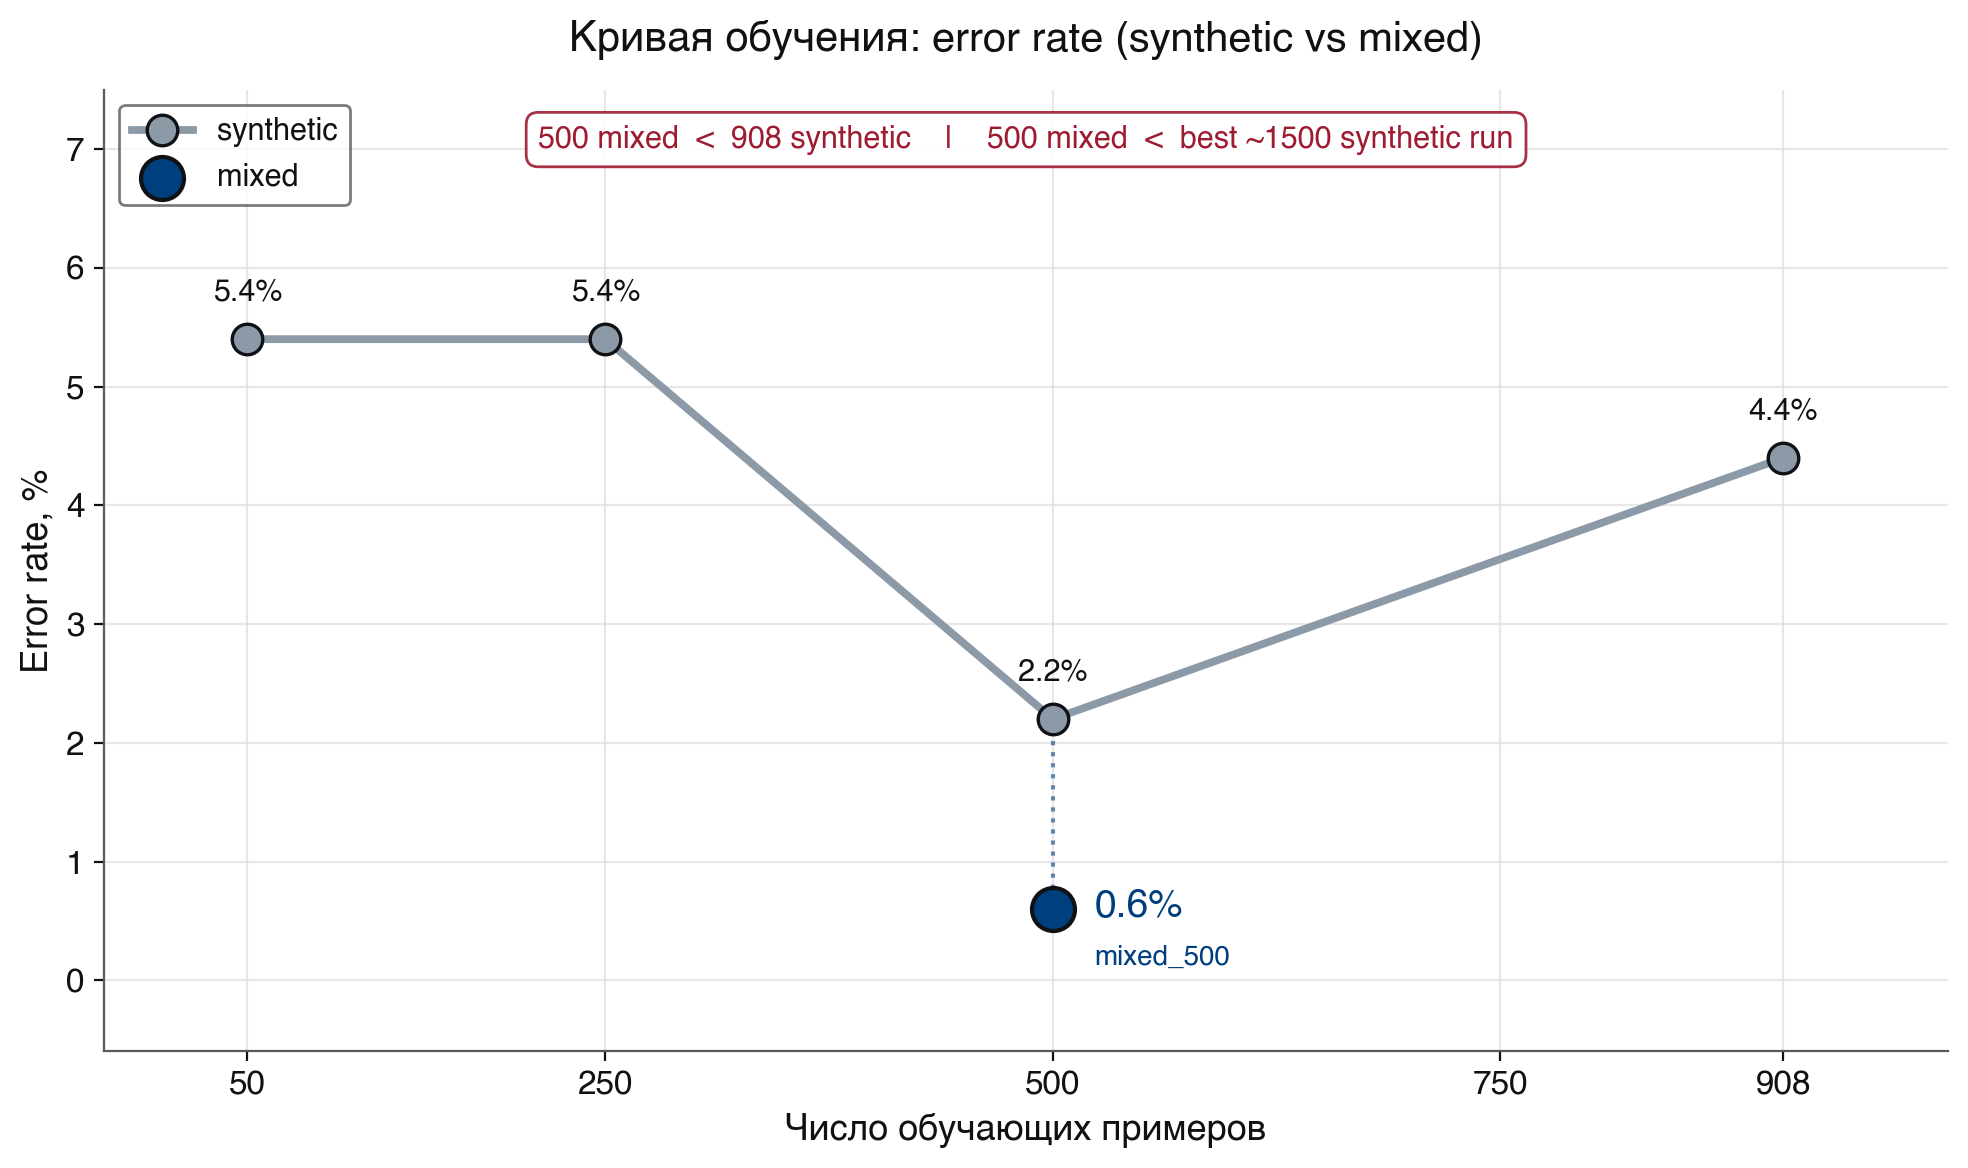
\includegraphics[width=0.9\textwidth]{figures/saturation_curve.png}
\caption{Кривая обучения: зависимость error rate и Macro~$F_1$ от объёма синтетических обучающих данных на \texttt{benchmark-combined}.}
\label{fig:saturation_curve}
\end{figure}

\begin{table}[H]
\centering
\caption{Confusion matrix модели \texttt{train\_synth\_50} на \texttt{benchmark-combined}. Строки~--- истинный класс, столбцы~--- предсказание модели; $n_{\varnothing}$~--- количество ответов без \texttt{tool\_call}.}
\label{tab:confusion_synth50}
\def\arraystretch{1.15}
\setlength\tabcolsep{0.5em}
\begin{tabular}{l r r r r}
    \toprule
    \textbf{Истинно \textbackslash{} Предсказано} & \texttt{ResolveEntities} & \texttt{SearchTags} & \texttt{GetSearchQuerySummary}$^{*}$ & $n_\varnothing$ \\
    \midrule
    \texttt{ResolveEntities} (GEO, 326) & 304 & 19 & 1 & 2 \\
    \texttt{SearchTags}\phantom{Resolve} (TAG, 174) & 4 & 169 & 1 & 0 \\
    \bottomrule
\end{tabular}\\[0.4em]
{\footnotesize $^{*}$~несуществующий инструмент, ошибочно сгенерированный моделью.}
\end{table}

%%% ============================================================
\subsection{Анализ типа обучающих данных} \label{subsec:data_type}
%%% ============================================================

Для проверки гипотезы~\ref{hyp:data_quality} сравним модели, обученные на данных различного типа при сопоставимых объёмах. Результаты сведены в таблице~\ref{tab:data_type_comparison}.

\begin{table}[H]
\centering
\caption{Сравнение моделей по типу обучающих данных (error rate $\downarrow$ лучше, Macro~$F_1$ $\uparrow$ лучше).}
\label{tab:data_type_comparison}
\def\arraystretch{1.15}
\setlength\tabcolsep{0.35em}
\begin{tabular}{l l r r r r}
    \toprule
    \textbf{Модель} & \textbf{Тип данных} & \multicolumn{2}{c}{\textbf{combined}} & \multicolumn{2}{c}{\textbf{real}} \\
    \cmidrule(lr){3-4} \cmidrule(lr){5-6}
     & & ER & M-F1 & ER & M-F1 \\
    \midrule
    train\_synth\_500  & Синтет.\,500  & $0{,}022$ & $0{,}979$ & $0{,}044$ & $0{,}942$ \\
    train\_real\_250   & Реал.\,250    & $0{,}048$ & $0{,}949$ & $0{,}020$ & $0{,}978$ \\
    train\_mixed\_500  & Микс\,500     & $0{,}006$ & $0{,}996$ & $0{,}012$ & $0{,}991$ \\
    \bottomrule
\end{tabular}
\end{table}

Наблюдается отчётливая специализация моделей по типу обучающих данных:
\begin{itemize}
    \item Модель на~синтетике (\texttt{train\_synth\_500}) превосходит модель на~реальных данных (\texttt{train\_real\_250}) на~смешанном бенчмарке ($\mathrm{ER}$ $0{,}022$ против $0{,}048$), но~уступает ей на~реальном ($0{,}044$ против $0{,}020$).
    \item \texttt{train\_real\_250} показывает лучший результат на \texttt{benchmark-real} ($\mathrm{ER} = 0{,}020$), но её error rate на \texttt{benchmark-combined} выше ($0{,}048$), поскольку синтетические примеры в тестовой выборке имеют иную структуру.
    \item \texttt{train\_mixed\_500} объединяет преимущества обоих типов данных и доминирует на обоих бенчмарках: $\mathrm{ER} = 0{,}006$ на combined и $0{,}012$ на real.
\end{itemize}

Данный результат подтверждает гипотезу~\ref{hyp:data_quality}: качество (разнородность и репрезентативность) обучающих данных оказывает большее влияние на итоговые метрики, чем их объём. Модель \texttt{train\_mixed\_500}, обученная на 500~примерах, превосходит все модели, обученные на ${\sim}\,1500$ синтетических примерах.

%%% ============================================================
\subsection{Анализ ошибок} \label{subsec:error_analysis}
%%% ============================================================

\subsubsection{Паттерны ошибок классификации}

Для каждой модели определены направления ошибок: GEO$\to$TAG (запрос GEO ошибочно классифицирован как TAG) и TAG$\to$GEO (запрос TAG ошибочно классифицирован как GEO). Результаты представлены в таблице~\ref{tab:error_patterns}.

\begin{table}[H]
\centering
\caption{Паттерны ошибок классификации на \texttt{benchmark-combined}}
\label{tab:error_patterns}
\def\arraystretch{1.15}
\setlength\tabcolsep{0.4em}
\begin{tabular}{l r r l}
    \toprule
    \textbf{Модель} & \textbf{G$\to$T} & \textbf{T$\to$G} & \textbf{Домин.\,ошибка} \\
    \midrule
    pro\_baseline$^{*}$ &  0 & 57 & TAG массово как GEO \\
    train\_synth\_*    &  8--24 &  1 & GEO массово как TAG \\
    train\_real\_250   &  1 & 21 & TAG$\to$GEO (дисбал.) \\
    train\_mixed\_500  &  0 &  1 & Практически нет \\
    \bottomrule
\end{tabular}\\[0.4em]
{\footnotesize $^{*}$~значение <<0 ошибок GEO$\to$TAG>> не отражает преимущества baseline: модель склонна по умолчанию предпочитать GEO, поэтому обратных ошибок не возникает. Кроме того, 34 запроса ($6{,}8\%$) не содержат \texttt{tool\_call} вовсе и не учтены в столбцах G$\to$T\,/\,T$\to$G.}
\end{table}

Обнаруживается характерная инверсия bias: базовая модель систематически классифицирует TAG-запросы как GEO, тогда как дообученные на синтетике модели совершают преимущественно обратную ошибку (GEO$\to$TAG). Это объясняется тем, что синтетические обучающие данные перепредставляют класс TAG, смещая решающую границу модели.

\begin{figure}[H]
\centering
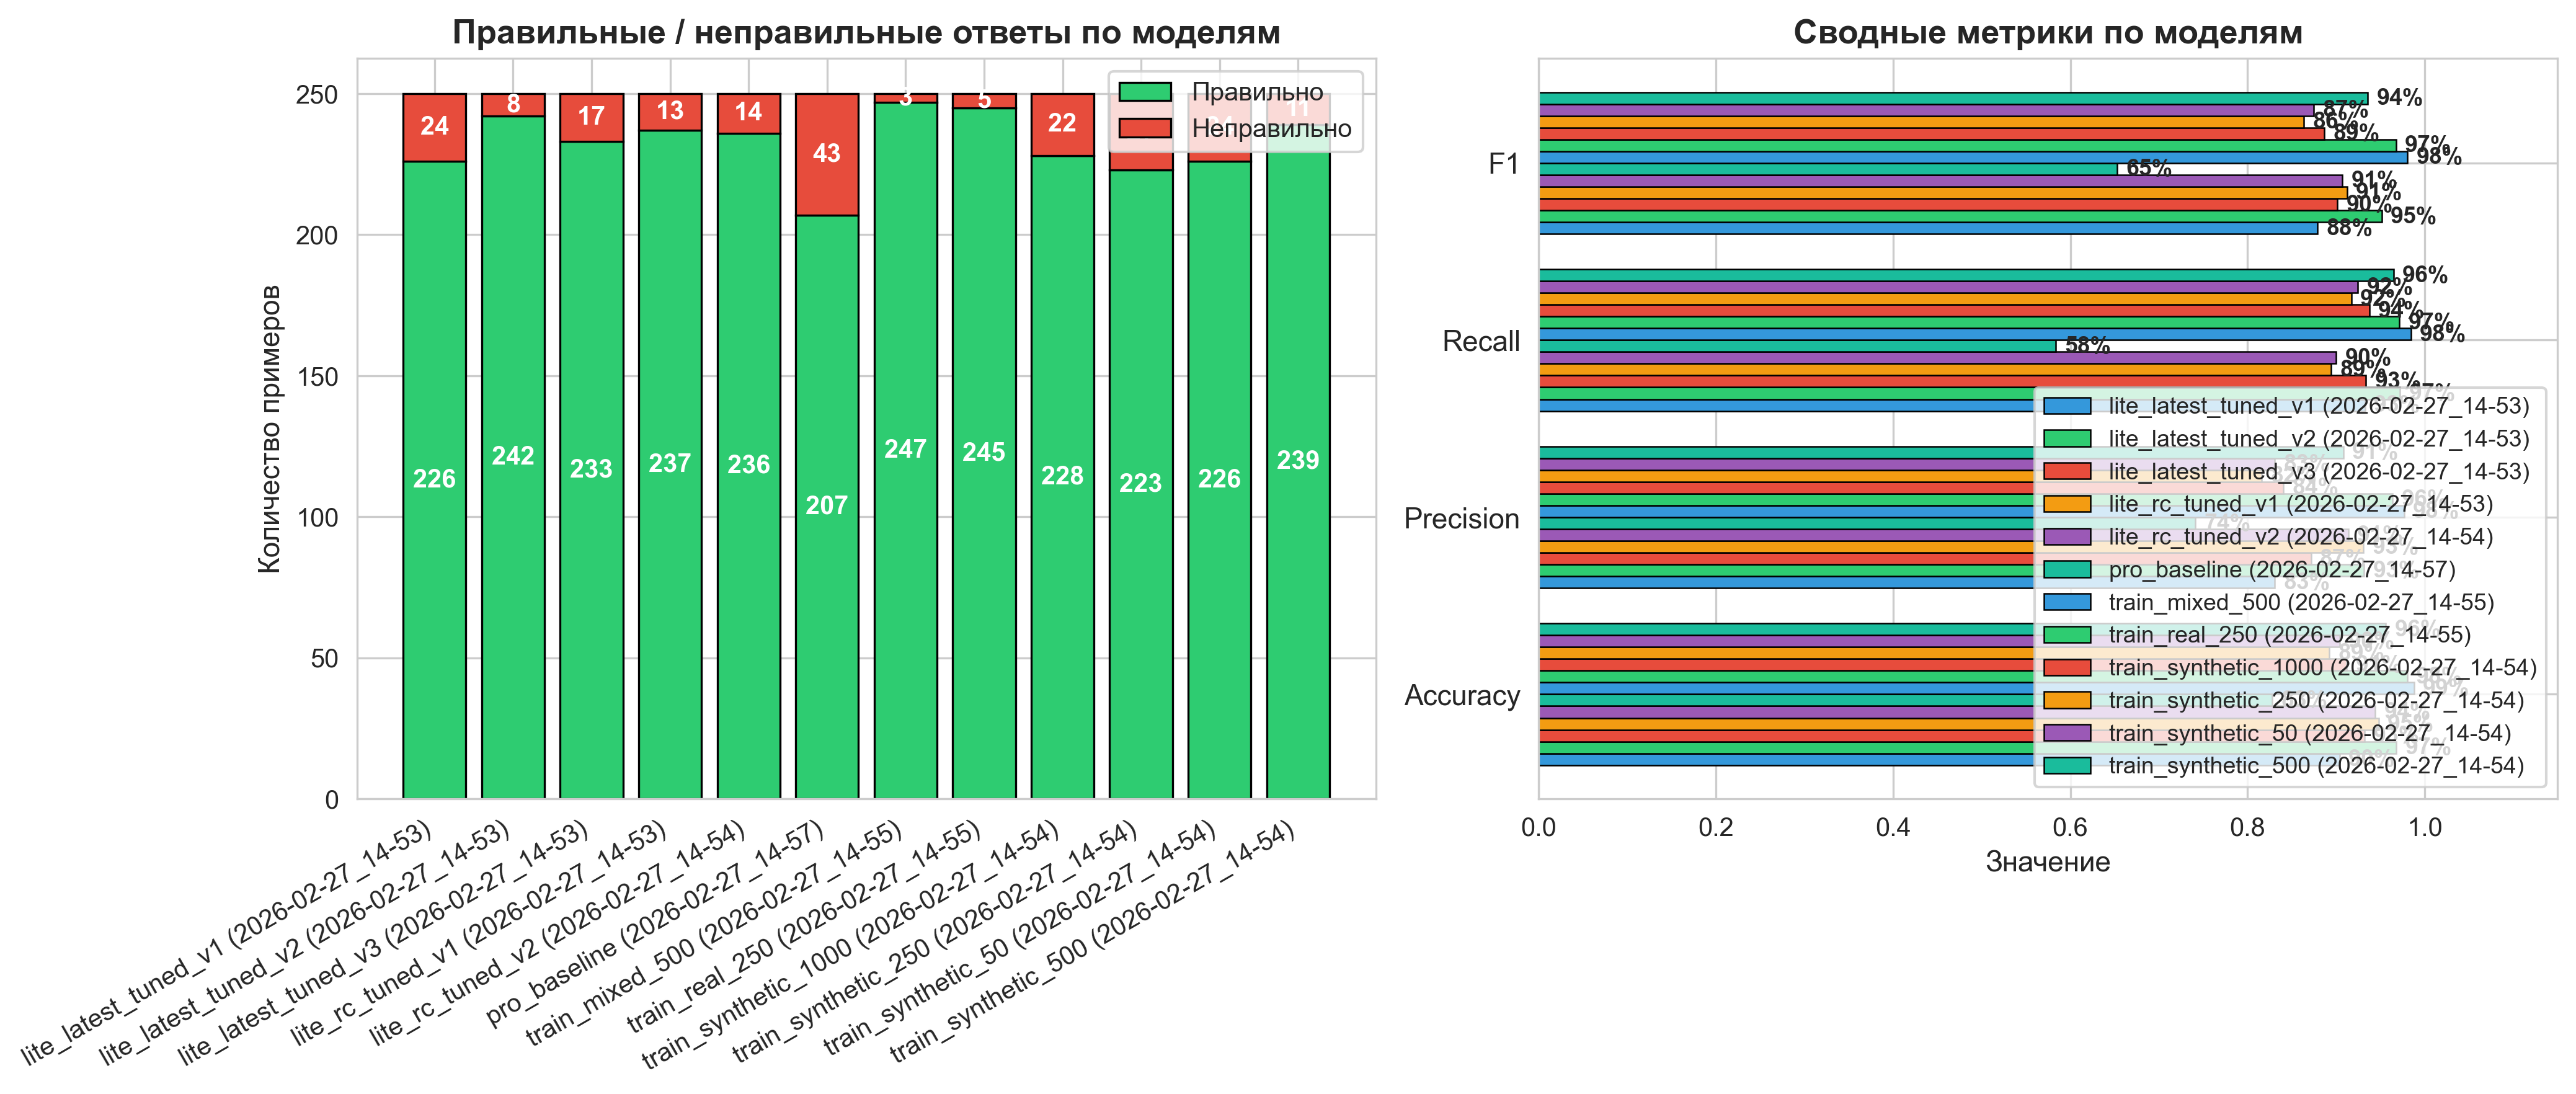
\includegraphics[width=\textwidth]{figures/group_per_model_errors.png}
\caption{Количество ошибок по моделям с разбиением по направлению (GEO$\to$TAG, TAG$\to$GEO, отказ) на обоих бенчмарках.}
\label{fig:per_model_errors}
\end{figure}

Модель \texttt{train\_mixed\_500} практически свободна от обоих типов bias (0~ошибок GEO$\to$TAG, 1~ошибка TAG$\to$GEO), что подтверждает эффективность сбалансированного микса данных для устранения систематических смещений.

\subsubsection{Консервация ошибок}

Анализ пересечения ошибок выявляет важный феномен: многие ошибки воспроизводимы~--- и на уровне одной модели (между бенчмарками), и между разными моделями.

\paragraph{Воспроизводимость между бенчмарками.} Для трёх показательных моделей (таблица~\ref{tab:error_conservation}) ошибки на \texttt{benchmark-real} в подавляющем большинстве совпадают с ошибками на \texttt{benchmark-combined}. Это означает, что ошибки обусловлены не стохастикой генерации, а систематическими слабостями модели на определённых типах запросов.

\begin{table}[H]
\centering
\caption{Консервация ошибок: совпадение ошибок на двух бенчмарках (combined\,/\,real)}
\label{tab:error_conservation}
\def\arraystretch{1.15}
\begin{tabular}{l c c}
    \toprule
    \textbf{Модель} & \textbf{GEO$\to$TAG} & \textbf{TAG$\to$GEO} \\
    \midrule
    lite\_latest\_v2   & 5\,/\,5 & 1\,/\,1 \\
    train\_synth\_500  & 8\,/\,8 & 1\,/\,1 \\
    train\_mixed\_500  & 0\,/\,0 & 1\,/\,1 \\
    \bottomrule
\end{tabular}
\end{table}

\paragraph{Распределение ошибок по 12 моделям.} На \texttt{benchmark-combined} из 500~примеров 368 ($73{,}6\%$) классифицированы правильно \emph{всеми} 12~моделями; ещё 78 ($15{,}6\%$) ошибочны лишь у одной модели. Ни один пример не ошибочен у всех 12 моделей~--- это означает, что каждый запрос принципиально решаем хотя бы одной из рассмотренных конфигураций. В то же время существует устойчивое <<трудное ядро>>: 9~примеров ошибочны у шести и более моделей, 3~примера~--- у одиннадцати из двенадцати (таблица~\ref{tab:error_distribution}).

\begin{table}[H]
\centering
\caption{Распределение примеров \texttt{benchmark-combined} по числу ошибающихся моделей}
\label{tab:error_distribution}
\def\arraystretch{1.15}
\setlength\tabcolsep{0.6em}
\begin{tabular}{r r r}
    \toprule
    \textbf{Ошиблось моделей} & \textbf{Кол-во примеров} & \textbf{\% от 500} \\
    \midrule
    0     & 368 & $73{,}6$ \\
    1     &  78 & $15{,}6$ \\
    2--3  &  35 & $7{,}0$ \\
    4--5  &  10 & $2{,}0$ \\
    6--8  &   6 & $1{,}2$ \\
    9--11 &   6 & $1{,}2$ \\
    12    &   0 & $0{,}0$ \\
    \bottomrule
\end{tabular}
\end{table}

\paragraph{Пересечение ошибочных множеств между моделями.} Коэффициент Жаккара между множествами ошибочных ответов двух моделей, $J(A, B) = |E_A \cap E_B| / |E_A \cup E_B|$, даёт меру близости их паттернов ошибок. Наиболее характерные наблюдения:
\begin{itemize}
    \item $J(\texttt{pro\_baseline},\,\cdot) \leqslant 0{,}17$ для всех дообученных моделей~--- ошибки baseline \emph{качественно отличны} от ошибок дообученных моделей (у baseline это TAG$\to$GEO, у дообученных~--- GEO$\to$TAG, см.~таблицу~\ref{tab:error_patterns}).
    \item $J(\texttt{lite\_rc\_v1},\,\texttt{lite\_rc\_v2}) = 0{,}77$~--- почти идентичные множества ошибок, что естественно для моделей одной итерации разработки.
    \item $J(\texttt{train\_synth\_50},\,\texttt{train\_synth\_1000}) = 0{,}58$~--- существенное совпадение ошибок у синтетических моделей разного объёма, подтверждающее, что артефакты синтетической генерации консервативны.
    \item $J(\texttt{train\_real\_250},\,\texttt{train\_mixed\_500}) = 0{,}12$~--- различные паттерны ошибок у моделей с реальными данными.
\end{itemize}

\paragraph{Лингвистический анализ <<трудного ядра>>.} Из 9~примеров, ошибочных у шести и более моделей, 8~относятся к классу GEO. Все они обладают одним или несколькими общими признаками (таблица~\ref{tab:hard_examples}):

\begin{table}[H]
\centering
\caption{Примеры <<трудного ядра>>: запросы, ошибочные у $\geqslant 9$ моделей из~12}
\label{tab:hard_examples}
\def\arraystretch{1.15}
\setlength\tabcolsep{0.3em}
{\small
\begin{tabular}{l l p{0.55\textwidth} c}
    \toprule
    \textbf{ID} & \textbf{True} & \textbf{Запрос} & \textbf{Ошиб.} \\
    \midrule
    q\_00159 & GEO & <<купить однокомнатную в центре Симферополя>>                    & 11 \\
    q\_00165 & TAG & <<кладовка от застройщика новый век>>                            & 11 \\
    q\_00253 & GEO & <<купить квартиру ялта ул красноармейская 13>>                   & 11 \\
    q\_00046 & GEO & <<ищу квартиру поближе к зелёной ветке и подешевле снять>>       &  9 \\
    q\_00473 & GEO & <<...с очень классным ремонтом..., в рамках ТТК, до 80\,000 руб.>> &  9 \\
    q\_00496 & GEO & <<снять студию с собакой в приморском районе...>>                 &  9 \\
    \bottomrule
\end{tabular}
}
\end{table}

Выделяются два систематических источника ошибок:
\begin{enumerate}
    \item \textbf{Жаргонные и абревиатурные топонимы.} <<Зелёная ветка>> (линия метро), <<ТТК>> (Третье транспортное кольцо), <<приморский район>> (имя собственное в нижнем регистре)~--- модели не распознают эти выражения как именованные сущности и склоняют их к классу TAG.
    \item \textbf{Длинные комплексные запросы с доминирующей TAG-составляющей.} В запросах типа q\_00473 и q\_00496 географическая привязка занимает менее $10\%$ длины запроса, а остальные признаки (ремонт, этажность, цена, наличие животного) воспринимаются как TAG-характеристики; модели следуют за доминантой.
\end{enumerate}

Обратный случай~--- q\_00165 (<<кладовка от застройщика новый век>>)~--- представляет собой ошибку противоположного типа: <<Новый век>> является потенциальным названием жилого комплекса, и модели ошибочно распознают его как имя собственное, относя запрос к GEO.

Выявленные паттерны соответствуют фундаментально неоднозначным случаям: безусловно корректная классификация требует внешней базы знаний (словарь имён собственных, справочник жилых комплексов), что выходит за пределы возможностей классификатора на основе LLM без RAG-компонента.

%%% ============================================================
\subsection{Статистическая значимость} \label{subsec:significance}
%%% ============================================================

\subsubsection{Критерий Кохрена}

Для проверки глобальной гипотезы о равенстве долей ошибок всех 12~моделей применён $Q$-критерий Кохрена (Cochran's~$Q$~test), являющийся обобщением критерия Макнемара на случай $k > 2$ связанных выборок (раздел~\ref{sec:background}):

\begin{itemize}
    \item \texttt{benchmark-combined}: $Q = 348{,}0$, $p < 10^{-6}$;
    \item \texttt{benchmark-real}: $Q = 128{,}8$, $p < 10^{-6}$.
\end{itemize}

На обоих бенчмарках нулевая гипотеза $H_0\colon \pi_1 = \pi_2 = \ldots = \pi_{12}$ отвергается при любом разумном уровне значимости. Следовательно, модели статистически значимо различаются по доле ошибок.

\subsubsection{Попарные сравнения (критерий Макнемара)}

Для попарного сравнения моделей применён точный критерий Макнемара. При $k = 12$ моделях число пар составляет $m = \binom{12}{2} = 66$, поэтому каждое получаемое $p$-значение сравнивается со скорректированным порогом $\alpha_{\mathrm{adj}} = 0{,}05 / 66 \approx 0{,}000758$ (поправка Бонферрони, раздел~\ref{subsubsec:bonferroni}). Различие признаётся статистически значимым только при $p \leqslant \alpha_{\mathrm{adj}}$; такая граница обеспечивает FWER не выше $0{,}05$ для всей серии 66~сравнений.

\paragraph{\texttt{benchmark-combined}.}
\begin{itemize}
    \item \texttt{train\_mixed\_500} статистически значимо превосходит большинство моделей ($p < \alpha_{\mathrm{adj}}$ для всех пар, кроме \texttt{lite\_latest\_v2}).
    \item Пара \texttt{lite\_latest\_v2} --- \texttt{lite\_rc\_v1} неразличима: $p = 0{,}73 \gg \alpha_{\mathrm{adj}}$.
\end{itemize}

\paragraph{\texttt{benchmark-real}.}
\begin{itemize}
    \item \texttt{train\_mixed\_500} и \texttt{train\_real\_250} статистически неразличимы: $p = 0{,}50$.
    \item Обе модели статистически значимо превосходят все модели, обученные исключительно на синтетических данных.
\end{itemize}

\begin{figure}[H]
\centering
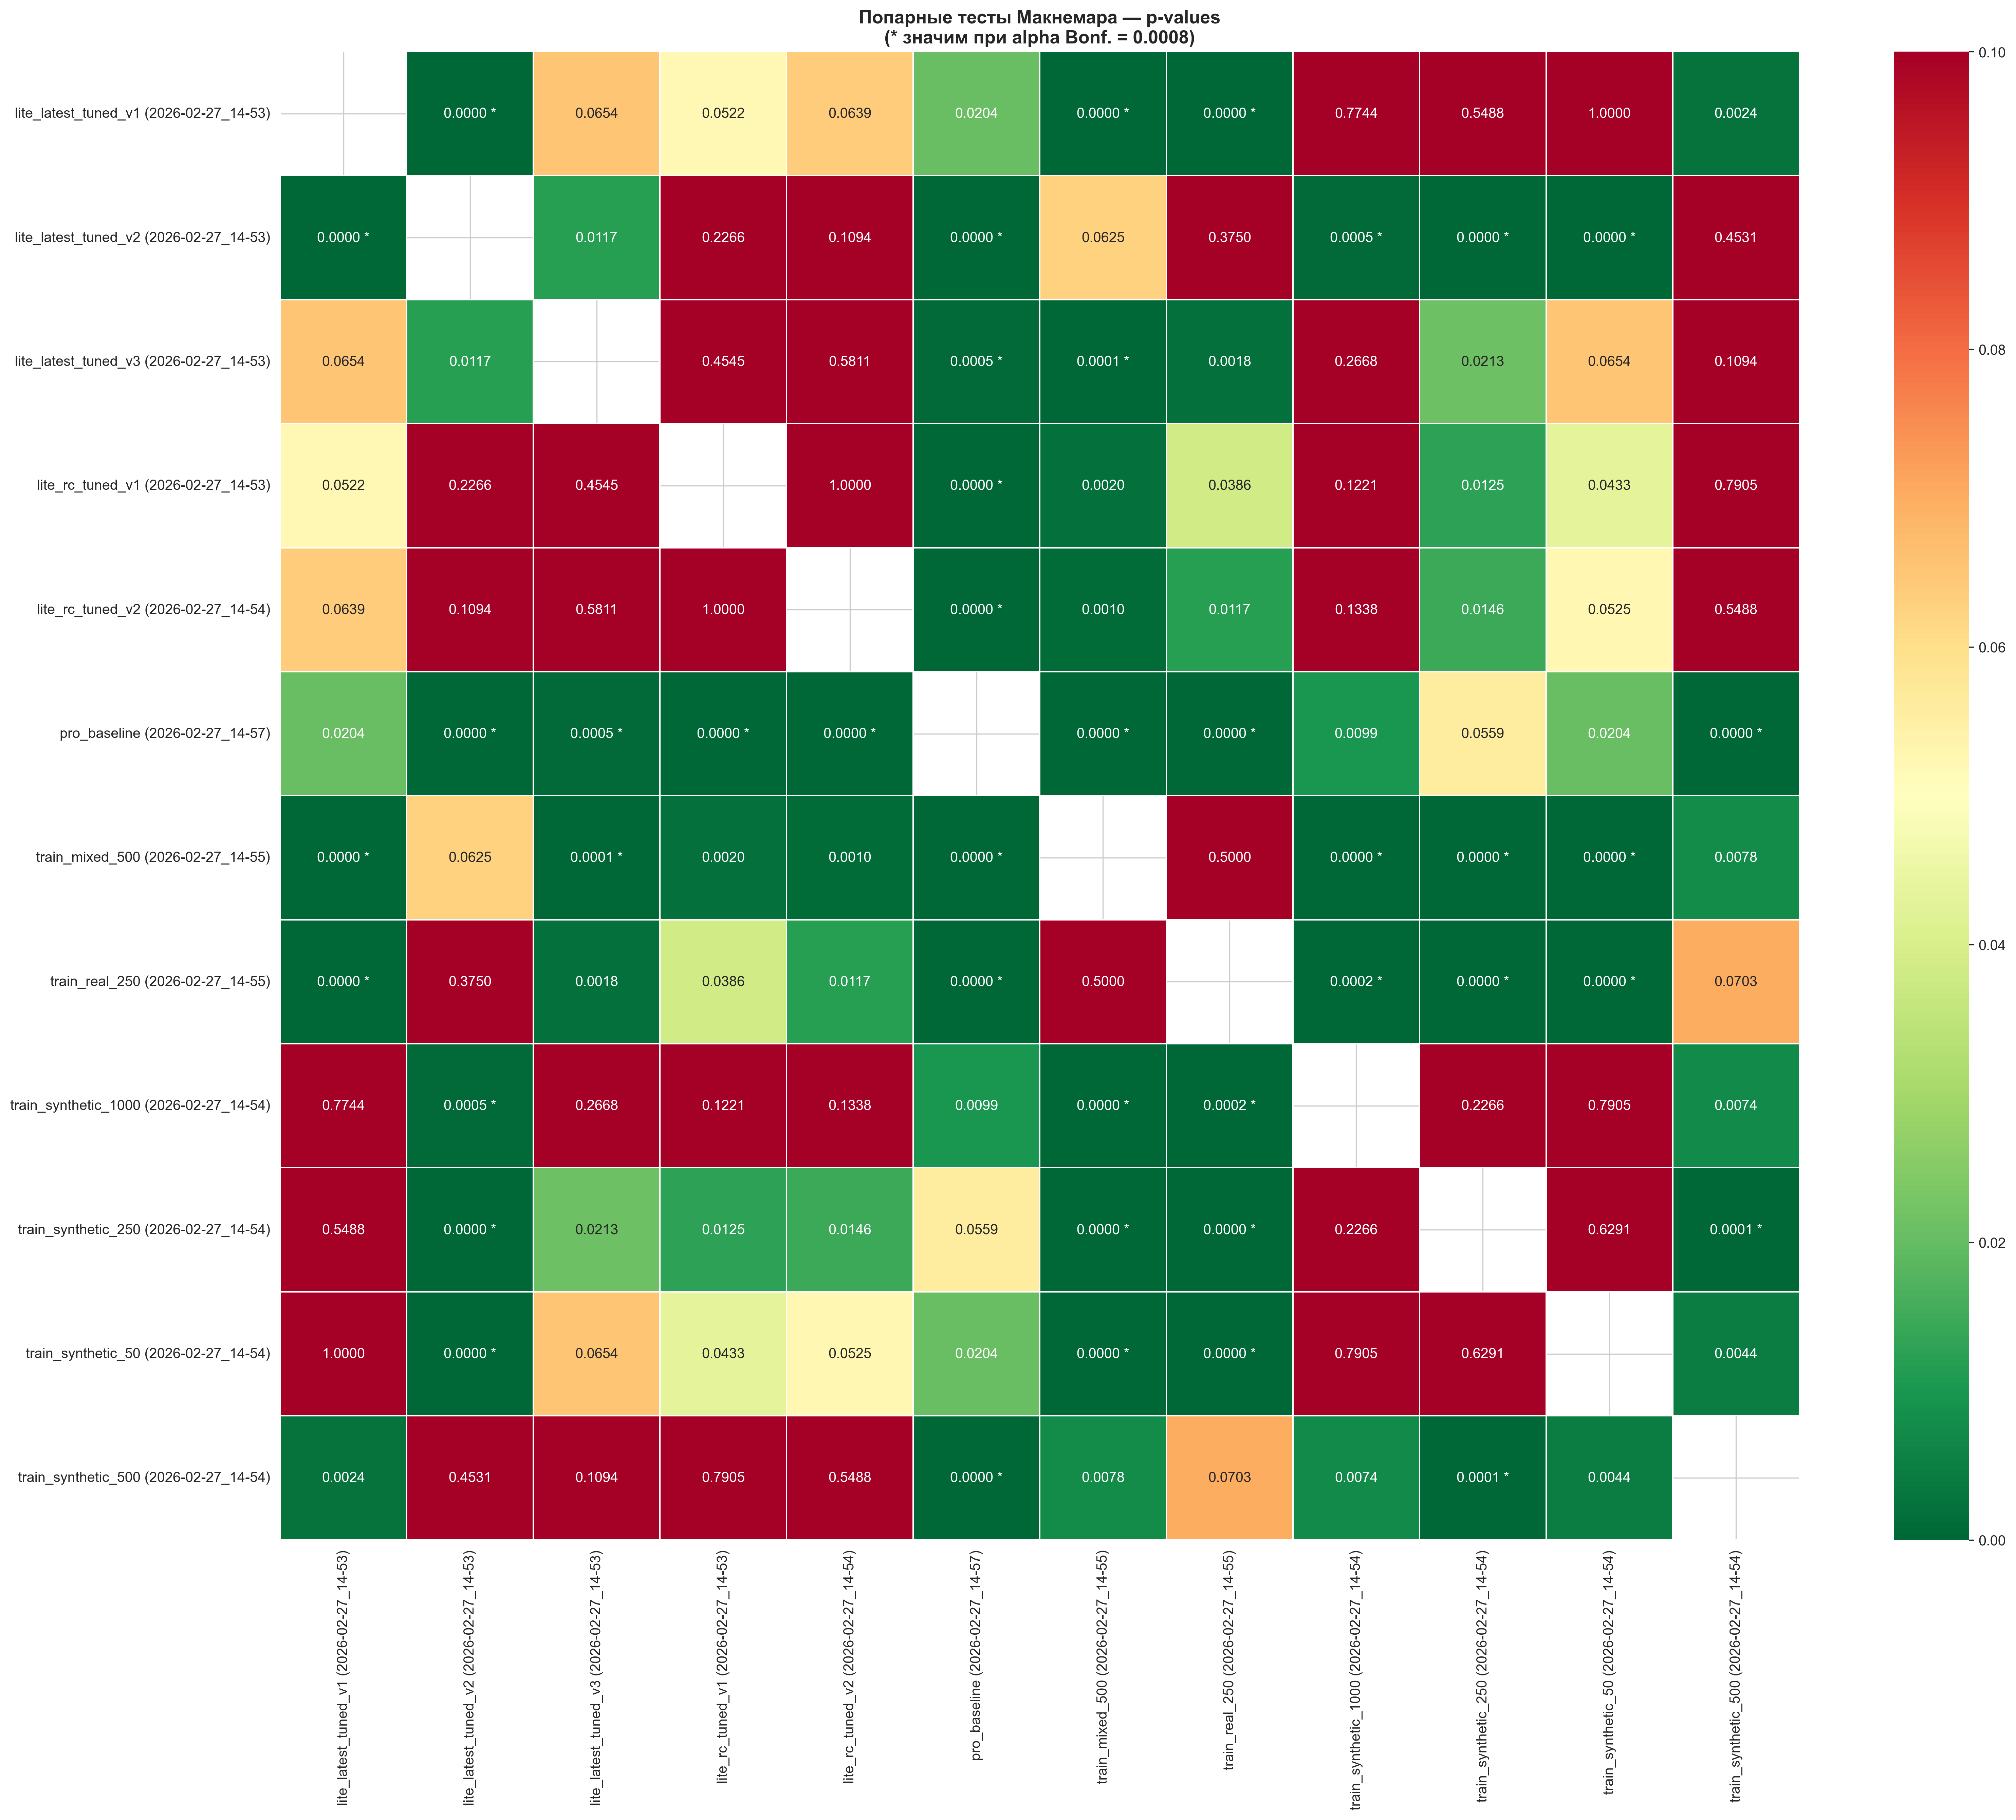
\includegraphics[width=0.95\textwidth]{figures/group_mcnemar_heatmap.png}
\caption{Тепловая карта $p$-значений попарного критерия Макнемара для 12~моделей на \texttt{benchmark-combined}. Тёмные ячейки~--- значимые различия ($p < \alpha_{\mathrm{adj}}$), светлые~--- неразличимые пары.}
\label{fig:mcnemar_heatmap}
\end{figure}

Данные результаты означают, что на реальных данных наличие реальных примеров в обучающей выборке является ключевым фактором: модель \texttt{train\_real\_250} (250~реальных примеров) статистически неотличима от \texttt{train\_mixed\_500} (500~смешанных), тогда как \texttt{train\_synth\_500} (500~синтетических) значимо уступает обеим.

\subsubsection{Согласованность предсказаний}

Анализ согласованности позволяет оценить долю примеров, на которых все 12~моделей дают одинаковый ответ:
\begin{itemize}
    \item \texttt{benchmark-combined}: $368$ из $500$ примеров ($73{,}6\%$) классифицированы правильно всеми 12~моделями; $0$~примеров ошибочны у всех~12.
    \item \texttt{benchmark-real}: $175$ из $250$ примеров ($70{,}0\%$) классифицированы правильно всеми 12~моделями.
\end{itemize}

Отсутствие примеров, ошибочных у всех 12~моделей, означает, что каждый запрос в бенчмарке в принципе решаем хотя бы одной из рассмотренных моделей. Оставшиеся ${\sim}\,27\text{--}30\%$ примеров составляют <<зону разногласий>>, где модели расходятся в предсказаниях, и именно на этих примерах сосредоточены различия в качестве.

%%% ============================================================
\subsection{Ответы на исследовательские вопросы} \label{subsec:rq_answers}
%%% ============================================================

\paragraph{\textsc{RQ1}: Каково влияние дообучения на метрики классификации?}

Дообучение методом LoRA приводит к статистически значимому улучшению всех метрик. Лучшая модель \texttt{train\_mixed\_500} снижает error rate с $0{,}182$ до $0{,}006$ (более чем в~$30$~раз; $-17{,}6$~п.п.) и повышает Macro~$F_1$ с $0{,}526$ до $0{,}996$ ($+0{,}470$). Даже наименее успешная дообученная модель (\texttt{lite\_latest\_v1}, $\mathrm{ER} = 0{,}072$) снижает error rate более чем в~$2{,}5$~раза по сравнению с baseline. Число отказов ($\rho_\varnothing$) снижается с $6{,}8\%$ до $0{,}4\%$ для всех дообученных моделей. Результат статистически значим по критерию Кохрена ($Q = 348{,}0$, $p < 10^{-6}$) и попарным критериям Макнемара.

\paragraph{\textsc{RQ2}: Как зависит качество от объёма обучающих данных?}

Зависимость немонотонна. При фиксированном типе данных (синтетика) error rate падает от $0{,}054$ (50~примеров) до минимума $0{,}022$ (500~примеров), после чего возрастает до~$0{,}044$ (908~примеров). Наиболее информативна динамика Macro~$F_1$: скачок с $0{,}631$ до $0{,}945$ при переходе от 50 к 250~примерам отражает исчезновение паразитного класса (раздел~\ref{subsec:learning_curve}); рост error rate при 908~примерах свидетельствует о переобучении на синтетическое распределение.

\paragraph{\textsc{RQ3}: Как тип обучающих данных влияет на робастность модели?}

Тип данных оказывает определяющее влияние. Модели на чистой синтетике демонстрируют рост error rate $+2{,}2\ldots +5{,}4$~п.п.\ при переходе на реальные данные. Модель \texttt{train\_real\_250} показывает обратный эффект: $-2{,}8$~п.п.\ на \texttt{benchmark-real} по сравнению с \texttt{benchmark-combined}. Оптимальная стратегия~--- смешанный датасет: \texttt{train\_mixed\_500} достигает $\mathrm{ER} \leqslant 0{,}012$ на обоих бенчмарках с деградацией всего $+0{,}6$~п.п. Это подтверждает гипотезу~\ref{hyp:data_quality}.

\paragraph{\textsc{RQ4}: Статистически значимы ли различия между моделями?}

Да. Критерий Кохрена отвергает гипотезу о равенстве моделей на обоих бенчмарках ($p < 10^{-6}$). Попарные сравнения Макнемара с поправкой Бонферрони ($\alpha_{\mathrm{adj}} \approx 0{,}0008$) показывают, что \texttt{train\_mixed\_500} значимо превосходит большинство моделей на \texttt{benchmark-combined}. На \texttt{benchmark-real} модели \texttt{train\_mixed\_500} и \texttt{train\_real\_250} статистически неразличимы ($p = 0{,}50$) и обе значимо лучше всех чисто синтетических моделей. Пара \texttt{lite\_latest\_v2}~--- \texttt{lite\_rc\_v1} также неразличима ($p = 0{,}73$).

\paragraph{Проверка гипотез H1a и H1b.} Гипотеза~\ref{hyp:lora_significance} (H1a) подтверждается попарным критерием Макнемара между \texttt{pro\_baseline} и любой дообученной моделью: $p \ll \alpha_{\mathrm{adj}}$. Гипотеза~\ref{hyp:lora_threshold} (H1b) подтверждается непосредственно: верхняя граница 95\%-го bootstrap-CI error rate для \texttt{train\_mixed\_500} на \texttt{benchmark-combined} составляет~$0{,}014$ (таблица~\ref{tab:combined_results}), что существенно меньше требуемого порога~$0{,}10$.

\clearpage
